\chapter{Sensor Linearity
\label{chap:10}}

To map the crushed gap sensor measurements to estimated forces, 
a regression to the forces as measured by the 
Linear Cutting Machine's strain gauges was used.
This method has a few limitations, the most significant
being the distance between the tested sensor and the strain gauges.
Because of the distance, the higher frequency force components will
be out of phase when compared. 
In addition to the distance, the viscous nature of the polyimide dielectric distorts the 
frequency response when the two measurements are compared.
The electronics for the sensor also contribute high frequency noise to the measurement.
For these reasons, the higher frequency components of the force are not directly correlated 
between the two systems. 
A plot of the transfer function between the measurements is shown in \ref{fig:sense_tf}.

The final sensor prototypes are shown in \ref{fig:airgap}.
When it comes to integrating this sensor with the target application,
construction of the sensor contributes to overall linear performance.
The steel case is assembled using the laser weld procedure described in \ref{app:laser}.
Simulation for the capacitance of the air gap is described in \ref{app:sim}.

The capacitive steel donut with viscous polyimide filling is a useful base design
for many robotic applications. Robustness, linearity, and sensitivity are important 
parameters for any sensor design. Ways to improve each of these categories is listed in \ref{tab:improve}.
To overcome the conflicting directions between sensitivity and the other design goals,
 use a thicker film and compress it down so that it becomes more thin and stiff.
Based on the other results in this work, high frequency classification 
should also be considered a valid method for
 determining material type and tool wear. 
Directly embedding a piezo element within the tool could
also serve to measure higher frequency vibrations which vary with cutting parameters.
Future works may be able to integrate the sensing membrane with the cutting tool,
using the tool to protect the sensor while it measures vibrations or cutting forces.


\begin{table}[]
\centering
\caption{Changes to design parameters that would improve certain categories}
\label{tab:improve}
\begin{tabular}{|r|c|c|c|}
\hline
Parameter               & Robustness   & Linearity    & Sensitivity               \\ \hline
Dielectric Thickness    & +            & +            & -   \\ \hline
Dielectric Stiffness    & +            & +            & -   \\ \hline
Dielectric Permittivity & No effect    & +            & +   \\ \hline
Case Walls Thickness    & +            & +            & -   \\ \hline
Sensing Electrode Area  & +            & +            & -   \\ \hline
\end{tabular}
\end{table}

\begin{figure}[ht]
\centering
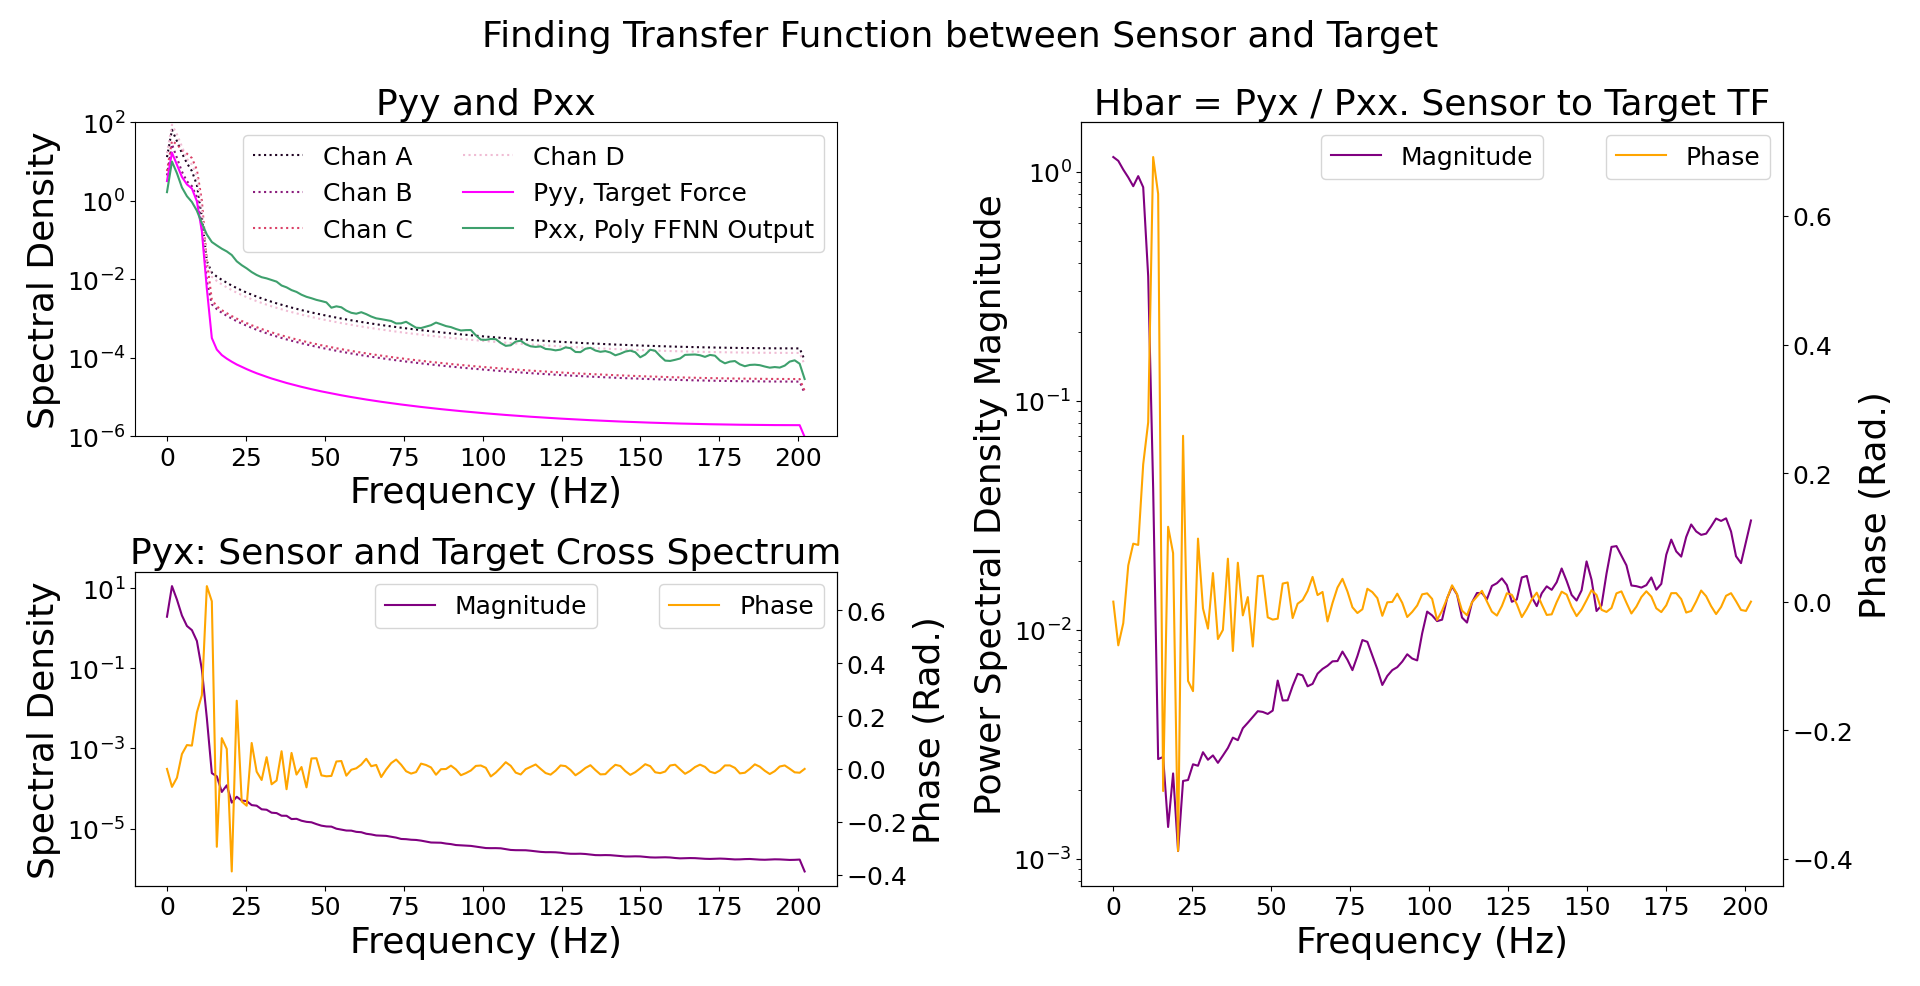
\includegraphics[width=5.5in]{ch10_tf.png}
\caption{
Power spectral density of sensor, target, and transfer function between them.
The regression target has been low pass filtered with a cutoff frequency of 10 Hz,
which can be seen by the steep drop in magnitude at this point.
The individual sensor channels have the same filter applied to limit high frequency input.
The cross spectrum, $P_{yx}$, shows that there is good correlation between the low frequency
components of the estimate and the target.
The transfer function between the estimate and the target suggests that additional 
filtering after the regression method could improve results.
Post-processing requirements depend on the application, and 
additional filtering after regression could be a useful technique for tuning performance.
}
\label{fig:sense_tf}
\end{figure}

\begin{figure}[ht]
\centering
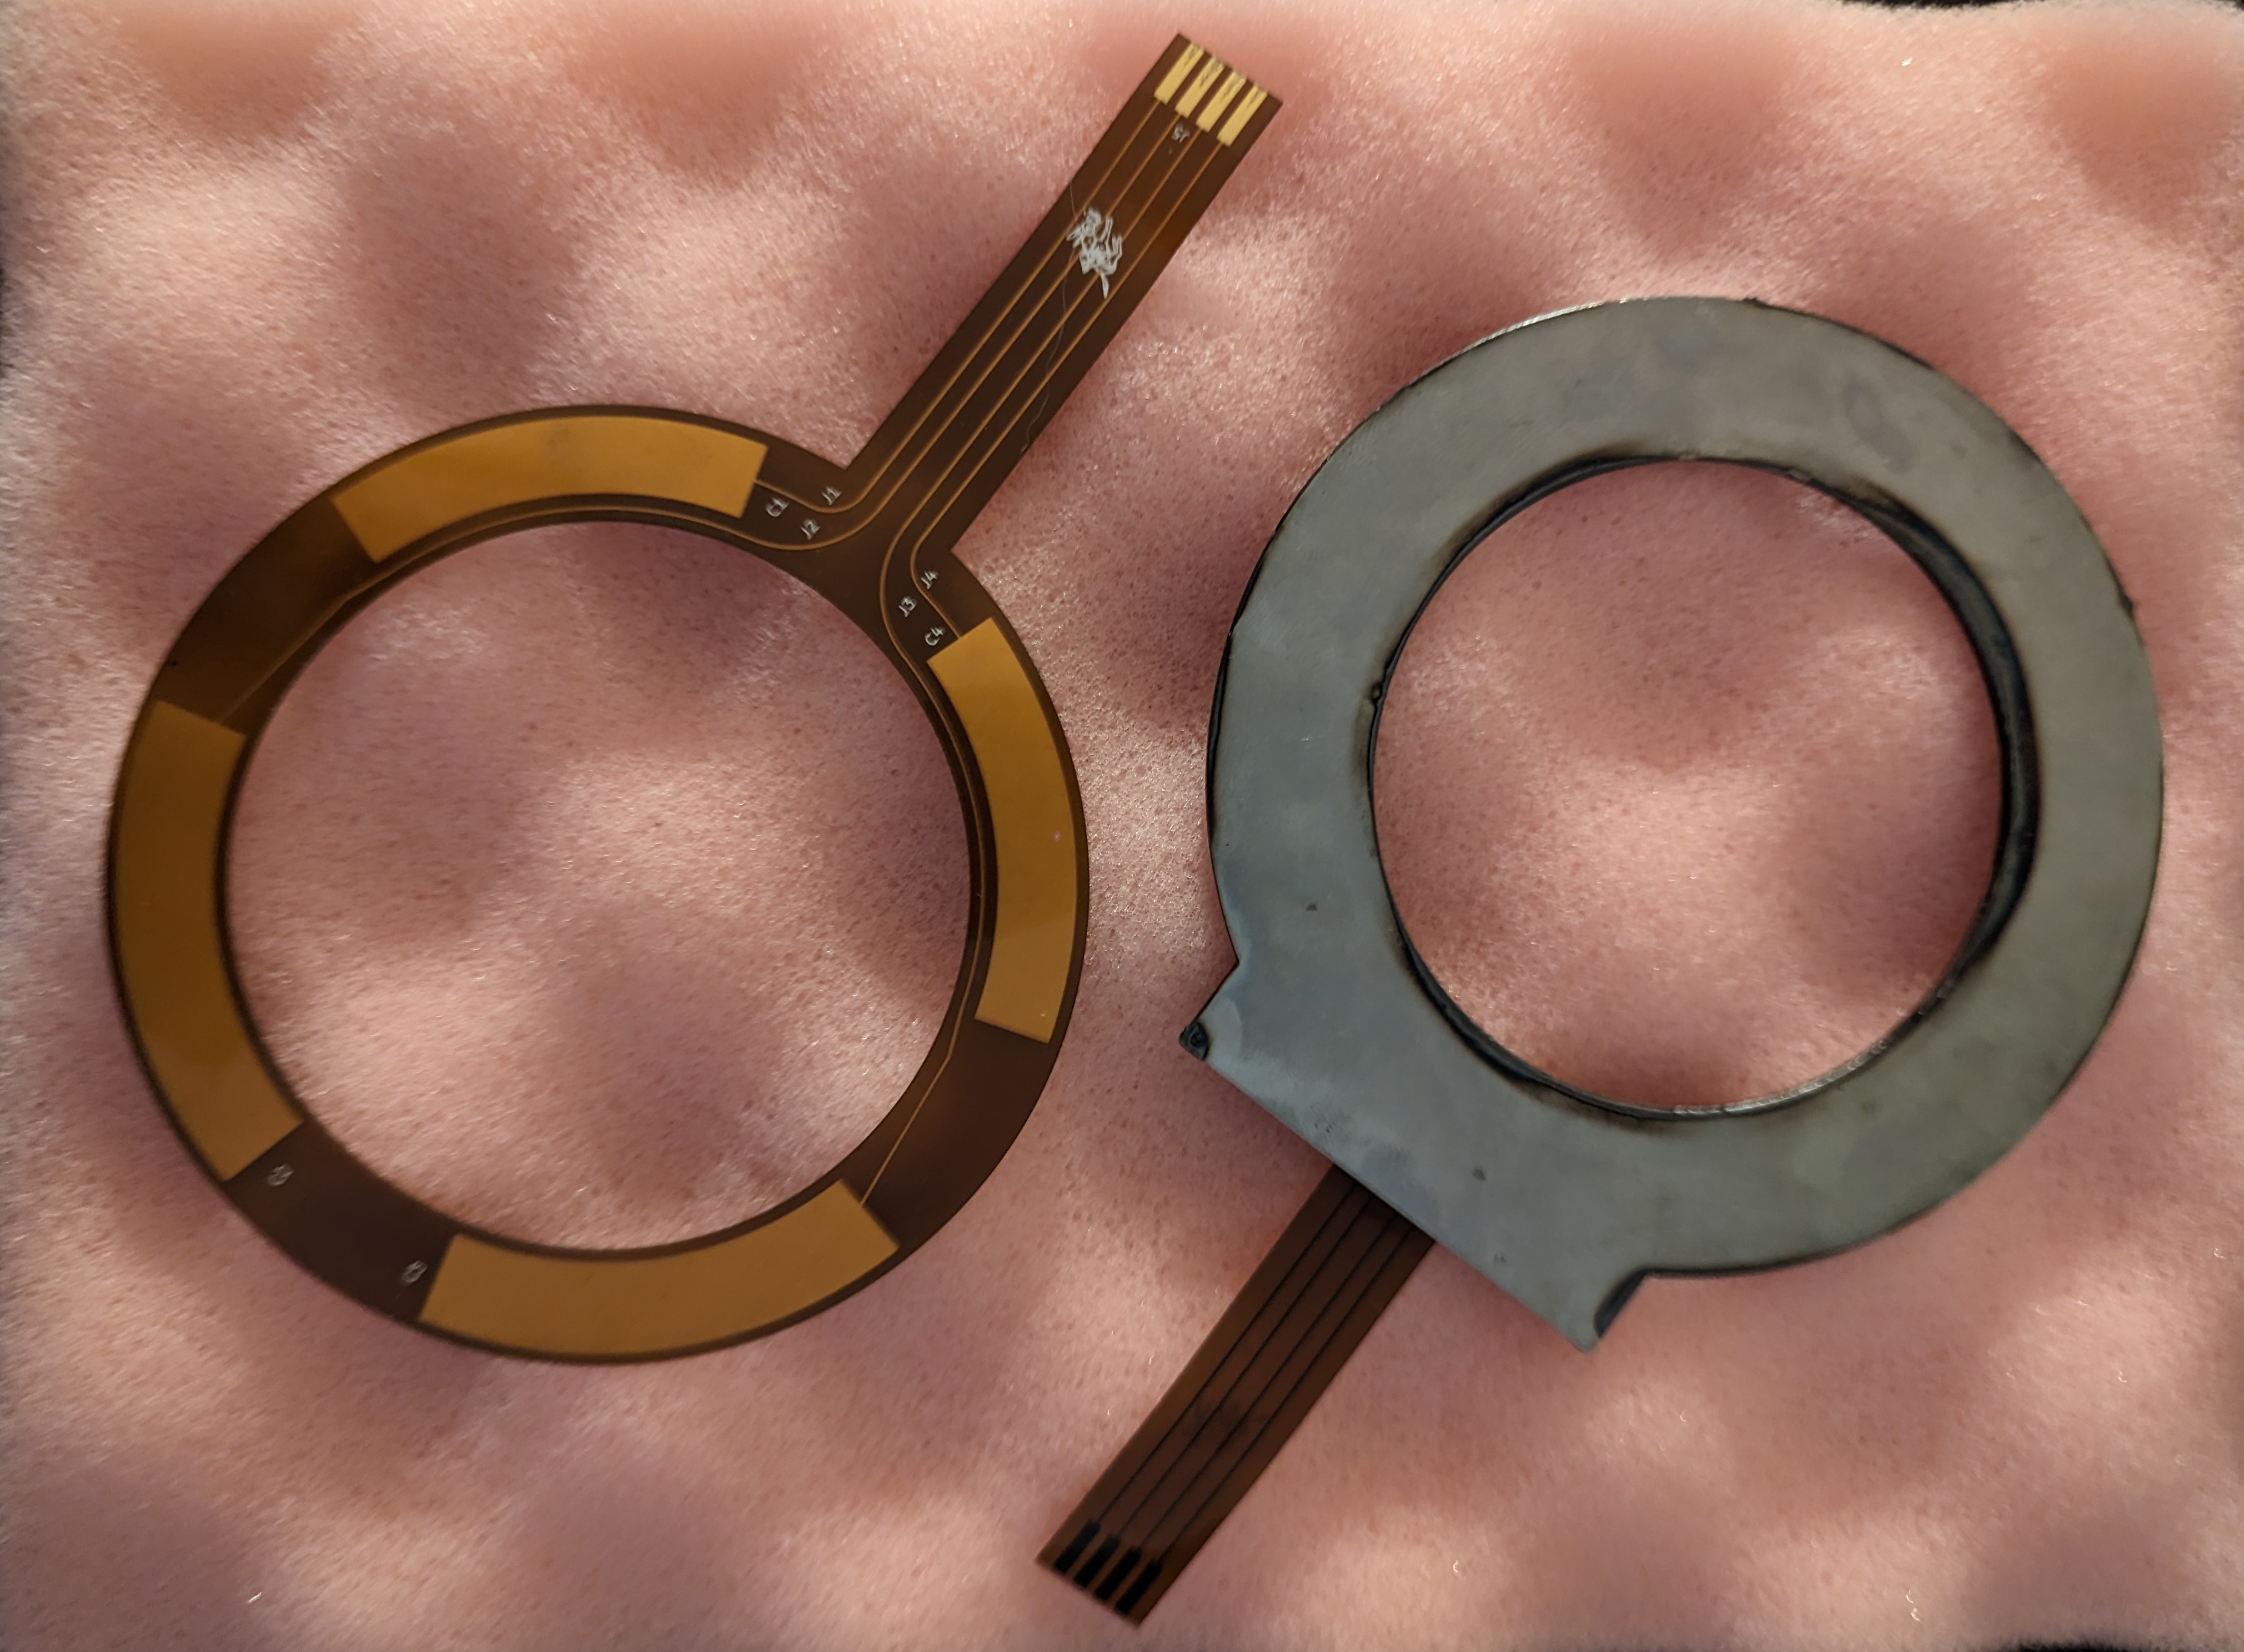
\includegraphics[width=0.5\textwidth]{ch10_airgap_and_case.jpg}
\caption{
The air gap sensor membrane, left, and an assembled prototype, right.
The sensor case provides additional protection from the environment.
The device is assembled via later welding.
Future sensor designs could omit the steel case and integrate the sensor directly within
the block or sleeve of the tool.
This type of sensor measures cutting forces via the change in capacitance caused
by the displacement of the top of the case when force is applied. 
}
\label{fig:airgap}
\end{figure}

